\documentclass[aspectratio=169,11pt]{beamer}
\usepackage[T1]{fontenc}
\usepackage{lmodern,amsmath,amssymb,mathtools,bm,booktabs,array,graphicx,tikz}
\usetikzlibrary{arrows.meta,positioning,calc,decorations.pathreplacing,patterns}
\definecolor{ink}{HTML}{17344D}\definecolor{accent}{HTML}{087E8B}\definecolor{pale}{HTML}{EDF5F5}\definecolor{gold}{HTML}{AD6B19}
\providecommand{\dd}{\,\mathrm{d}}\providecommand{\R}{\mathbb{R}}
\providecommand{\E}{\mathbb{E}}\providecommand{\Var}{\operatorname{Var}}
\providecommand{\Cov}{\operatorname{Cov}}\providecommand{\diag}{\operatorname{diag}}
\providecommand{\norm}[1]{\left\lVert#1\right\rVert}
\providecommand{\abs}[1]{\left|#1\right|}
\usefonttheme{professionalfonts}
\setbeamercolor{normal text}{fg=black,bg=white}
\setbeamercolor{frametitle}{fg=ink,bg=white}
\setbeamercolor{title}{fg=ink}\setbeamercolor{structure}{fg=accent}
\setbeamercolor{block title}{fg=ink,bg=pale}\setbeamercolor{block body}{fg=black,bg=pale!40}
\setbeamercolor{alerted text}{fg=accent}
\setbeamerfont{frametitle}{size=\Large,series=\bfseries}
\setbeamerfont{title}{size=\LARGE,series=\bfseries}
\setbeamertemplate{navigation symbols}{}
\setbeamersize{text margin left=.7cm,text margin right=.7cm}
\setbeamertemplate{frametitle}{\vspace{.18cm}\insertframetitle\par\vspace{.1cm}{\color{accent}\hrule height .6pt}\vspace{.12cm}}
\newcommand{\notestarget}{notes.pdf}\newcommand{\noteslabel}{Notes}
\setbeamertemplate{footline}{\hspace{.7cm}\color{ink}\scriptsize Mathematical Modeling\quad\href{\notestarget}{\noteslabel}\hfill\insertframenumber\,/\,\inserttotalframenumber\hspace{.7cm}\vspace{.18cm}}
\setbeamercovered{invisible}
\hypersetup{pdfauthor={Zan Ahmad},pdftitle={A mixed chamber: differential equations and numerical stability},pdfpagemode=UseNone}
\begin{document}
\begin{frame}[plain]\vfill
{\small\color{accent} Mathematical Modeling \quad Lecture 3}\par\medskip
{\raggedright\hyphenpenalty=10000\exhyphenpenalty=10000\LARGE\bfseries\color{ink} A mixed chamber: differential equations and numerical stability}\par\bigskip
Zan Ahmad\par\smallskip
{\small Fall 2024}\par\vfill\end{frame}
\renewcommand{\notestarget}{notes.pdf\#note-concentration-and-the-removal-law}
\begin{frame}[t,fragile,label=slide-mixing-and-mass-outflow]{Mixing and mass outflow}
\[c=M/W,\qquad Qc=(Q/W)M.\]\pause{} Define $k=Q/W$ and mass input $r$.\[\dot M=r-kM.\]
\end{frame}
\renewcommand{\notestarget}{notes.pdf\#note-equilibrium-and-the-integrating-factor}
\begin{frame}[t,fragile,label=slide-equilibrium-and-direction-of-motion]{Equilibrium and direction of motion}
\[M_*=r/k,\qquad\dot M=k(M_*-M).\]\pause{} For $r=2$, $k=.25$, the equilibrium is $8$ mg. Below it the mass rises; above it the mass falls.
\end{frame}
\renewcommand{\notestarget}{notes.pdf\#note-equilibrium-and-the-integrating-factor}
\begin{frame}[t,fragile,label=slide-integrating-factor-derivation]{Integrating-factor derivation}
Let $e=M-M_*$. Then $\dot e=-ke$.\pause{}\[\frac{d}{dt}(e^{kt}e)=0\quad\Rightarrow\quad e(t)=e(0)e^{-kt}.\]
\end{frame}
\renewcommand{\notestarget}{notes.pdf\#note-equilibrium-and-the-integrating-factor}
\begin{frame}[t,fragile,label=slide-convex-combination-form]{Convex-combination form}
\[M(t)=e^{-kt}M_0+(1-e^{-kt})M_*.\]\pause{} Nonnegative weights summing to one imply positivity and confinement between the two endpoints.
\end{frame}
\renewcommand{\notestarget}{notes.pdf\#note-equilibrium-and-the-integrating-factor}
\begin{frame}[t,fragile,label=slide-relaxation-time-and-dimensionless-equation]{Relaxation time and dimensionless equation}
\[\tau=1/k,\quad\theta=kt,\quad m=M/M_*\quad(r>0).\]\pause{}\[dm/d\theta=1-m.\]After one $\tau$, departure is multiplied by $e^{-1}$.
\end{frame}
\renewcommand{\notestarget}{notes.pdf\#note-forward-euler-as-a-quadrature-approximation}
\begin{frame}[t,fragile,label=slide-euler-from-an-integral-balance]{Euler from an integral balance}
\[M(t+h)-M(t)=\int_t^{t+h}(r-kM(s))\,ds.\]\pause{}\[M_{n+1}=M_n+h(r-kM_n).\]The quadrature uses the old removal rate.
\end{frame}
\renewcommand{\notestarget}{notes.pdf\#note-forward-euler-as-a-quadrature-approximation}
\begin{frame}[t,fragile,label=slide-one-half-minute-step]{One half-minute step}
$M_n=4$, $r=2$, $k=.25$, $h=.5$.\[M_{n+1}=4+.5(2-.25\cdot4)=4.5.\]\pause{}\[M(t+h)=8-4e^{-.125}\approx4.4700.\]
\end{frame}
\renewcommand{\notestarget}{notes.pdf\#note-forward-euler-as-a-quadrature-approximation}
\begin{frame}[label=slide-continuous-and-discrete-filling-figure]{Continuous and discrete filling}
\centering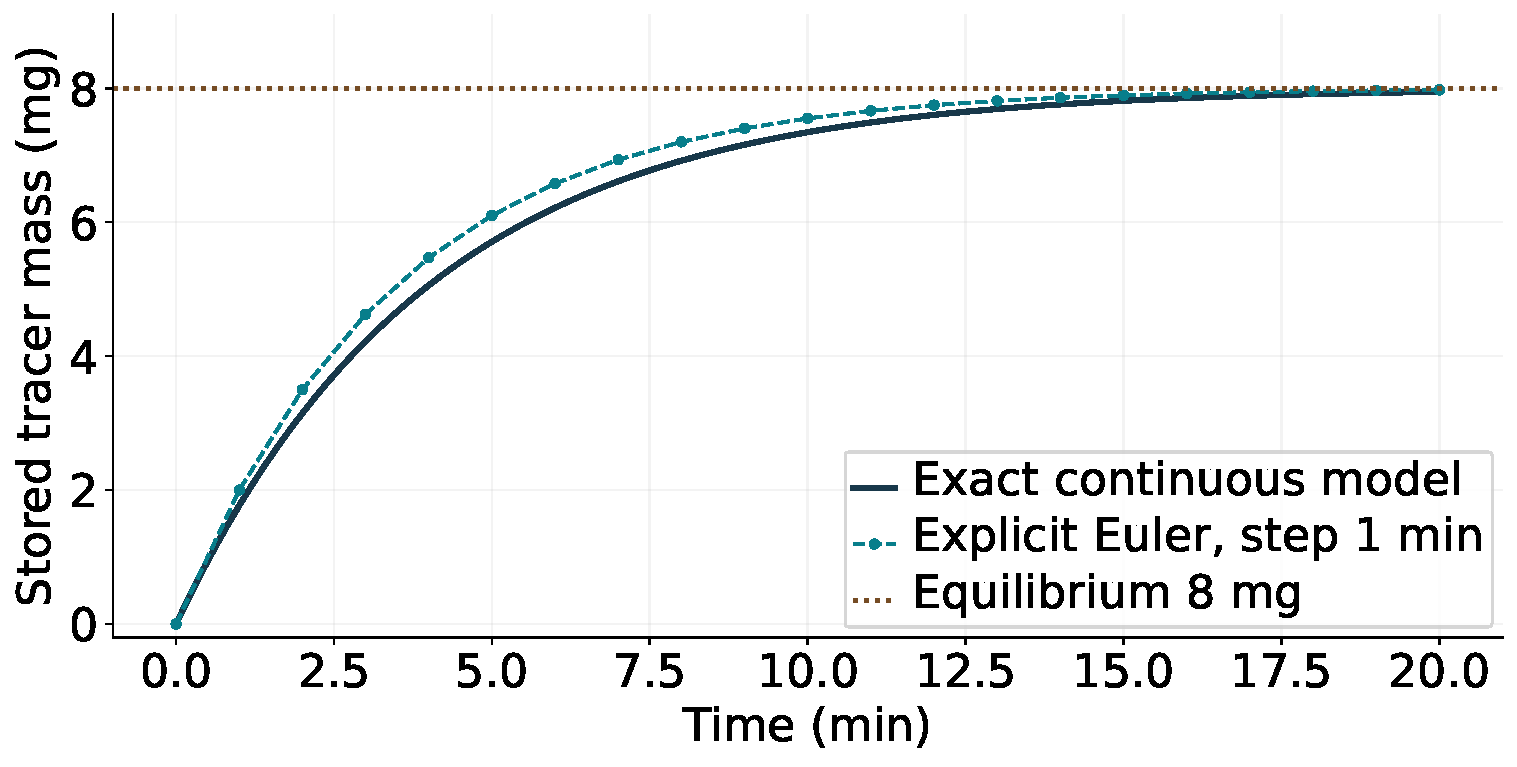
\includegraphics[width=.98\linewidth,height=.69\textheight,keepaspectratio]{presentation-figures/filling.pdf}\end{frame}
\renewcommand{\notestarget}{notes.pdf\#note-forward-euler-as-a-quadrature-approximation}
\begin{frame}[t,fragile,label=slide-continuous-and-discrete-filling]{Continuous and discrete filling}
\[M(t)=8(1-e^{-.25t}),\qquad M_n=8(1-.75^n)\quad(h=1).\]\pause{} The equilibrium agrees; finite-time trajectories differ.
\end{frame}
\renewcommand{\notestarget}{notes.pdf\#note-the-discrete-amplification-factor}
\begin{frame}[t,fragile,label=slide-exact-discrete-recurrence]{Exact discrete recurrence}
\[e_n=M_n-M_*,\quad e_{n+1}=(1-kh)e_n.\]\pause{}\[e_n=(1-kh)^ne_0.\]A negative multiplier alternates the side of equilibrium.
\end{frame}
\renewcommand{\notestarget}{notes.pdf\#note-the-discrete-amplification-factor}
\begin{frame}[t,fragile,label=slide-stability-interval]{Stability interval}
\[|1-kh|<1\Longleftrightarrow0<kh<2.\]\pause{} The subinterval $1<kh<2$ is stable but oscillatory.
\end{frame}
\renewcommand{\notestarget}{notes.pdf\#note-the-discrete-amplification-factor}
\begin{frame}[t,fragile,label=slide-positivity-of-the-euler-update]{Positivity of the Euler update}
\[M_{n+1}=(1-kh)M_n+hr.\]\pause{} For $M_n,r\geq0$, $0\leq kh\leq1$ guarantees a nonnegative result.
\end{frame}
\renewcommand{\notestarget}{notes.pdf\#note-large-step-trajectories-and-time-refinement}
\begin{frame}[label=slide-large-step-failure-modes-figure]{Large-step failure modes}
\centering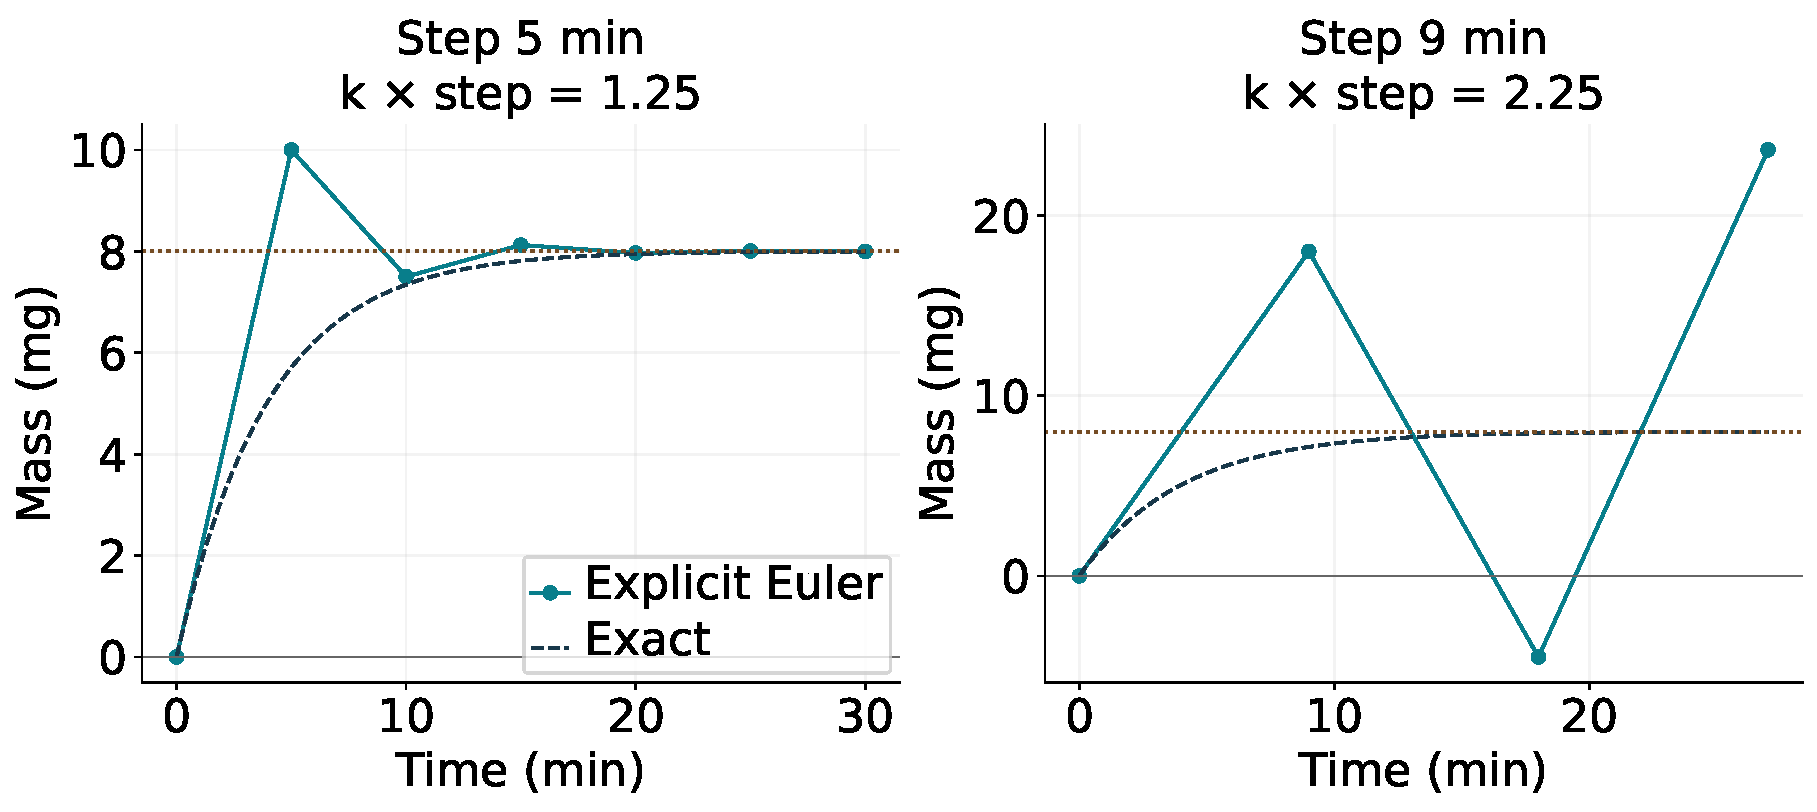
\includegraphics[width=.98\linewidth,height=.69\textheight,keepaspectratio]{presentation-figures/step-size.pdf}\end{frame}
\renewcommand{\notestarget}{notes.pdf\#note-large-step-trajectories-and-time-refinement}
\begin{frame}[t,fragile,label=slide-large-step-failure-modes]{Large-step failure modes}
$h=5$: $a=-.25$, sequence $0,10,7.5,8.125$.\pause{}\par $h=9$: $a=-1.25$, sequence $0,18,-4.5,23.625$.
\end{frame}
\renewcommand{\notestarget}{notes.pdf\#note-large-step-trajectories-and-time-refinement}
\begin{frame}[t,fragile,label=slide-fixed-time-refinement]{Fixed-time refinement}
\[E(h)=|M_h(T)-M(T)|,\qquad E(h)/E(h/2)\to2.\]\pause{} Match final time, initial condition, and physical parameters.
\end{frame}
\renewcommand{\notestarget}{notes.pdf\#note-large-step-trajectories-and-time-refinement}
\begin{frame}[t,fragile,label=slide-zero-removal-and-small-k-evaluation]{Zero removal and small-k evaluation}
$k=0$ gives $M=M_0+rt$.\pause{}\par Near zero evaluate $M_0e^{-kt}+r[-\operatorname{expm1}(-kt)/k]$, branching at exactly zero.
\end{frame}
\renewcommand{\notestarget}{notes.pdf\#note-a-conserved-discrete-account-can-conceal-instability}
\begin{frame}[t,fragile,label=slide-discrete-mass-budget]{Discrete mass budget}
\[D_{n+1}=D_n+hkM_n\quad\Rightarrow\quad M_n+D_n=M_0+rt_n.\]\pause{} The identity can hold even for negative computed mass.
\end{frame}
\renewcommand{\notestarget}{notes.pdf\#note-a-conserved-discrete-account-can-conceal-instability}
\begin{frame}[t,fragile,label=slide-numerical-and-physical-discrepancies]{Numerical and physical discrepancies}
Compare first with the exact equation solution, then with independent observations.\pause{}\par A small numerical error does not establish the mixing or proportional-removal assumptions.
\end{frame}
\end{document}
